\section{Specific Requirements}
Text
\subsection{External interface requirements}
Text
\subsubsection{User interfaces}


\begin{figure}[h!]
    \centering
    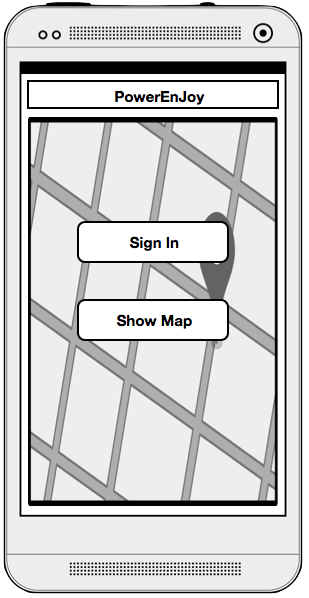
\includegraphics[scale=0.3]{{Figures/Mockup/1FirstScreen.png}}
    \label{fig:1FirstScreen}
    \\From the first screen a user can either sign in, or create a new account if he is a new user, or consult the map of available Cars.
\end{figure}

\begin{figure}[h!]
    \centering
    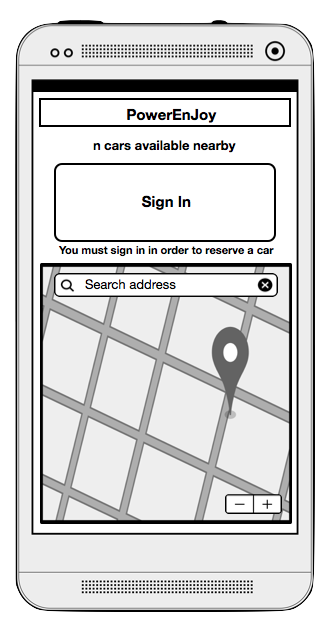
\includegraphics[scale=0.3]{{Figures/Mockup/2MapNotLogged.png}}
    \label{fig:2MapNotLogged}
    \\If a user chooses the map, he will see a map with all the available cars and he will be asked to sign in in order to proceed with the reservation.
\end{figure}


\begin{figure}[p!]
    \centering
    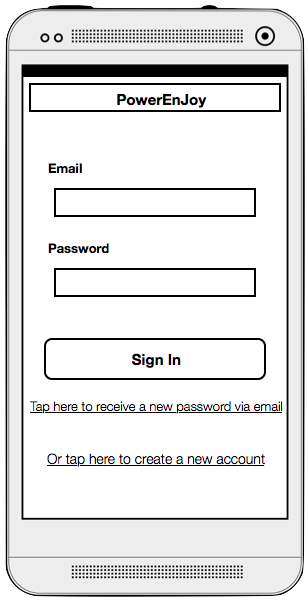
\includegraphics[scale=0.3]{{Figures/Mockup/3LoginForm.png}}
    \label{fig:3LoginForm}
    \\Whether a user started from the map or from the first screen, he will have to either enter his credential or register. In case of forgotten credential he is given the possibility to ask for a new password too.
\end{figure}

\begin{figure}[p!]
    \centering
    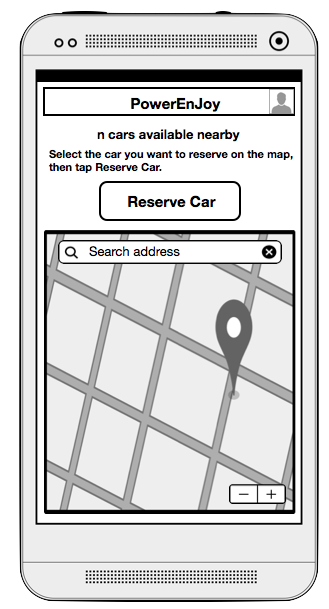
\includegraphics[scale=0.3]{{Figures/Mockup/4CarReservationA}}
    \label{fig:4CarReservationA}
    \\A PowerUser can look for a suitable Car nearby his position, or entering an adress in the appropriate bar above the map. After finding a Car the PowerUser can reserve it.
\end{figure}

\begin{figure}[p!]
    \centering
    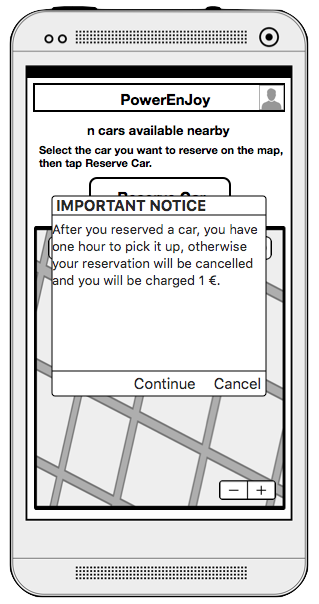
\includegraphics[scale=0.3]{{Figures/Mockup/4CarReservationB.png}}
    \label{fig:4CarReservationB}
    \\Before actually reserving a Car, the system reminds the PowerUser about the one hour expiration of his reservation and the relative penalty fee.
\end{figure}

\begin{figure}[p!]
    \centering
    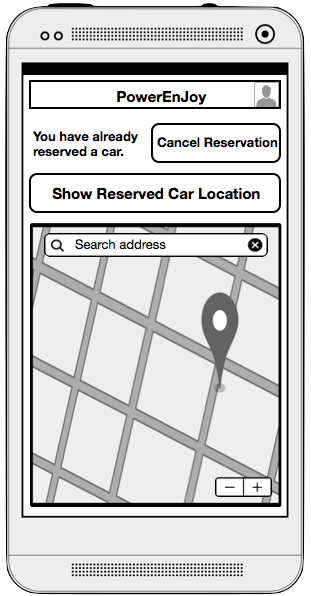
\includegraphics[scale=0.3]{{Figures/Mockup/5CarReserved.png}}
    \label{fig:5CarReserved}
    \\The selected Car has been reserved. Now a PowerUser can cancel his reservation or look for his car thanks to the provided map.
\end{figure}

\begin{figure}[p!]
    \centering
    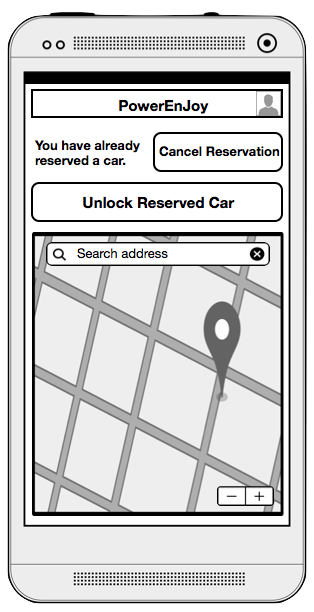
\includegraphics[scale=0.3]{{Figures/Mockup/6CarNearby.png}}
    \label{fig:6CarNearby}
    \\When a PowerUser is near his reserved Car, he is given the possibility to ask the system to unlock it. If the PowerUser changes his mind he can still cancel the reservation, this possibility will remain valid until the PowerUser ignites the engine. 
\end{figure}

\begin{figure}[p!]
    \centering
    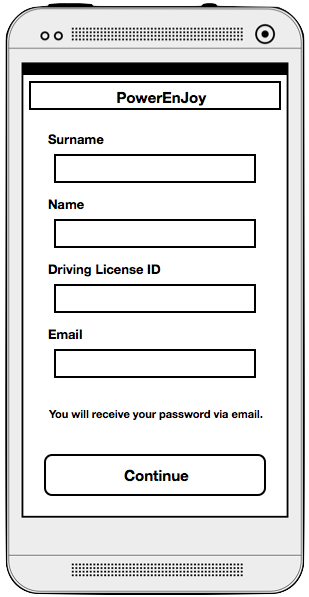
\includegraphics[scale=0.3]{{Figures/Mockup/7RegistrationFormA.png}}
    \label{fig:7RegistrationFormAForm}
    \\This is the first page that requires a new user to enter his personal data.
\end{figure}

\begin{figure}[p!]
    \centering
    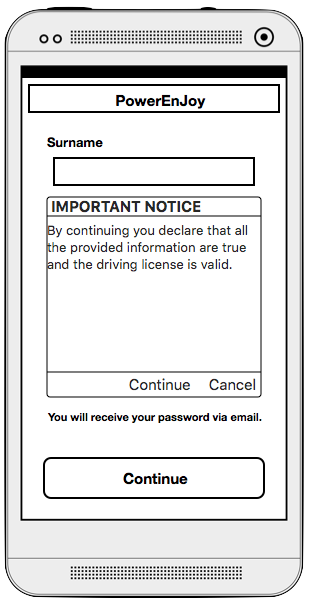
\includegraphics[scale=0.3]{{Figures/Mockup/7RegistrationFormB.png}}
    \label{fig:7RegistrationFormB}
    \\In order to stress the importance for the user to enter real and correct data, the system reminds the user about this.
\end{figure}

\begin{figure}[p!]
    \centering
    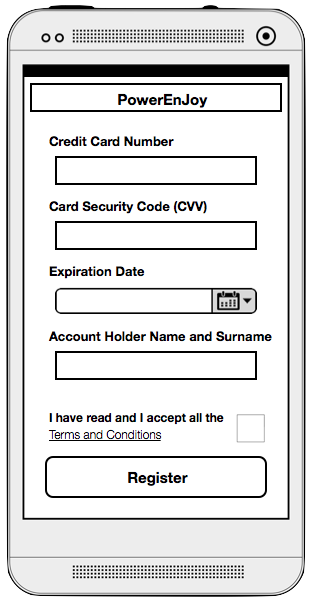
\includegraphics[scale=0.3]{{Figures/Mockup/7RegistrationFormC.png}}
    \label{fig:7RegistrationFormCnForm}
    \\Last page of the registration form, the user is asked for his payment information. Furthermore he will have to accept the terms and conditions of the service in order to complete the registration.
\end{figure}

\begin{figure}[p!]
    \centering
    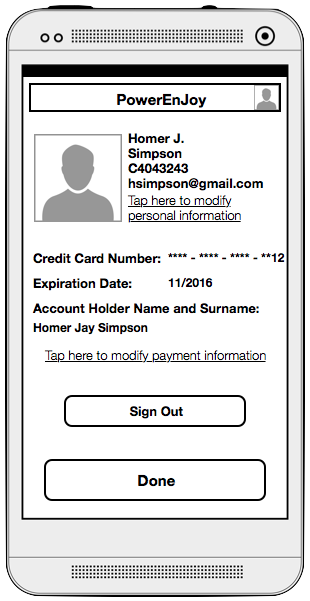
\includegraphics[scale=0.3]{{Figures/Mockup/8PersonalAccountPage.png}}
    \label{fig:8PersonalAccountPage}
    \\A PowerUser can access his personal account page by tapping on the avatar in the up right corner of his screen. By doing so, this is what he will be shown. From this page it is also possible to modify both personal and payment information.
\end{figure}

\begin{figure}[p!]
    \centering
    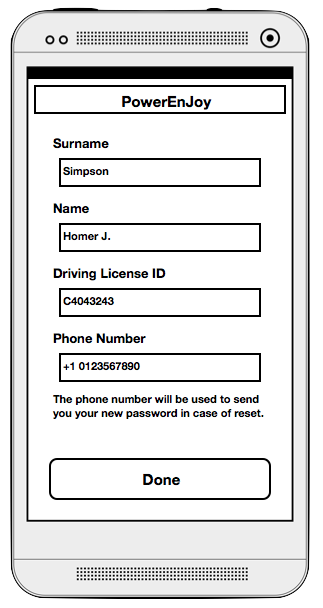
\includegraphics[scale=0.3]{{Figures/Mockup/9PersonalDataModification.png}}
    \label{fig:9PersonalDataModification}
    \\This is the page to be used by a PowerUser in order to modify his personal information.
\end{figure}

\begin{figure}[h!]
    \centering
    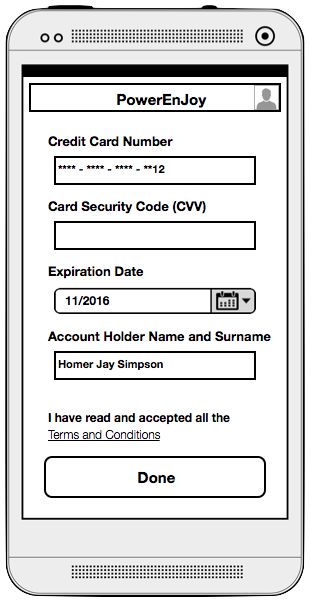
\includegraphics[scale=0.3]{{Figures/Mockup/10PaymentSystemDataModification.png}}
    \label{fig:10PaymentSystemDataModificationForm}
    \\This is the page to be used by a PowerUser in order to modify his payment information.
\end{figure}

\subsubsection{Hardware interfaces}
Text
\subsubsection{Communication interfaces}
Text
\subsubsection{Software interfaces}
Text
\subsection{Functional requirements}

\newcounter{goalctr}
    \stepcounter{goalctr}
    \subsubsection{Goal \arabic{goalctr}}
    {[}G\arabic{goalctr}{]}
    Allow any kind of user to view the map of the available nearby Cars
    \begin{itemize}
        \item Requirements
        \begin{enumerate}[label={[}R\arabic*{]},series=REQ]
    		\item Users must have access to a map indicating the user current location.
    		\item Users must be able to pan and scroll the map in any direction.
    		\item Every available Car must be shown on a map.
        \end{enumerate}
        \item Domain properties
        \begin{enumerate}[label={[}P\arabic*{]},series=PRO]
    			\item No Car with less than B\% battery charge is taken into account as available for booking.
    			\item No Car that is currently under charging and has less than C\% battery charge is taken into account as available for booking.
        \end{enumerate}
    \end{itemize}
    
    \stepcounter{goalctr}
    \subsubsection{Goal \arabic{goalctr}}
    {[}G\arabic{goalctr}{]}
    Allow Visitor user to register to the service.
    \begin{itemize}
        \item Requirements
        \begin{enumerate}[REQ]
    		\item Let a Visitor user start the registration wizard while he's still not logged in.
			\item The registration form must contain input fields for user identity, email, contact info, driving license number and expiration, privacy agreement confirmation, customer notifications and subscriptions options, credit card number and expiration, billing identity.
			\item The chosen email address must not be already used by another PowerUser.
			\item The credit card must be verified not to be blocked or expired upon registration.
			\item The user must receive a system generated password to the registered email address.
        \end{enumerate}
        \item Domain properties
        \begin{enumerate}[PRO]
    			\item None
        \end{enumerate}
    \end{itemize}

    \stepcounter{goalctr}
    \subsubsection{Goal \arabic{goalctr}}
    {[}G\arabic{goalctr}{]}
    Allow Visitor user to log-in and out as a PowerUser.
    \begin{itemize}
        \item Requirements
        \begin{enumerate}[REQ]
			\item A Visitor user must always see an input to access log-in form as long as he's still not logged in.
		    \item An input to perform log-out must always be available to the PowerUser if he's currently logged in.
        \end{enumerate}
        \item Domain properties
        \begin{enumerate}[PRO]
    			\item None
        \end{enumerate}
    \end{itemize}

    \stepcounter{goalctr}
    \subsubsection{Goal \arabic{goalctr}}
    {[}G\arabic{goalctr}{]}
    Allow PowerUser to check the status of the Car.
    \begin{itemize}
        \item Requirements
        \\For each Car shown to the PowerUser, he must be able to access information regarding:
        \begin{enumerate}[REQ]
    		\item remaining battery charge
			\item current position
        \end{enumerate}
        \item Domain properties
        \begin{enumerate}[PRO]
    			\item None
        \end{enumerate}
    \end{itemize}

    \stepcounter{goalctr}
    \subsubsection{Goal \arabic{goalctr}}
    {[}G\arabic{goalctr}{]}
    Allow PowerUser to reserve a Car.
    \begin{itemize}
        \item Requirements
        \begin{enumerate}[REQ]
    		\item The PowerUser must have the ability to start the reservation wizard for any available Car.
			\item The PowerUser must see a reminder about unfulfilled reservation penalty before confirmation.
			\item Show an input to allow the PowerUser to confirm and finalize the reservation.
        \end{enumerate}
        \item Domain properties
        \begin{enumerate}[PRO]
    			\item None
        \end{enumerate}
    \end{itemize}

    \stepcounter{goalctr}
    \subsubsection{Goal \arabic{goalctr}}
    {[}G\arabic{goalctr}{]}
	Allow PowerUser to check the position of the reserved car.
    \begin{itemize}
        \item Requirements
        \begin{enumerate}[REQ]
    	    \item As long as a reservation exists for the PowerUser an input must be available to give him the position of that Car on the map.
        \end{enumerate}
        \item Domain properties
        \begin{enumerate}[PRO]
    		\item None
        \end{enumerate}
    \end{itemize}

    \stepcounter{goalctr}
    \subsubsection{Goal \arabic{goalctr}}
    {[}G\arabic{goalctr}{]}
	Allow PowerUser to unlock and enter the Car when inside the specific range.
    \begin{itemize}
        \item Requirements
        \begin{enumerate}[REQ]
    	    \item The system must be able to remotely unlock the Car.
			\item The system must be able to compute the distance between the user location and his reserved Car.
			\item Show an input to the PowerUser allowing to send an unlock request.
        \end{enumerate}
        \item Domain properties
        \begin{enumerate}[PRO]
    			\item None
        \end{enumerate}
    \end{itemize}
    
    \stepcounter{goalctr}
    \subsubsection{Goal \arabic{goalctr}}
    {[}G\arabic{goalctr}{]}
    Allow PowerUser to get driving directions to his destination.
    \begin{itemize}
        \item Requirements
        \begin{enumerate}[REQ]
    			\item The user must be allowed to select a custom destination and start navigating to that location.
        \end{enumerate}
        \item Domain properties
        \begin{enumerate}[PRO]
    			\item Navigation software always provides effective directions to the user if destination it's included in Safe Areas.
        \end{enumerate}
    \end{itemize}

    \stepcounter{goalctr}
    \subsubsection{Goal \arabic{goalctr}}
    {[}G\arabic{goalctr}{]}
    Allow PowerUser to see a list of the closest Special Parking Areas to his destination.
    \begin{itemize}
        \item Requirements
        \begin{enumerate}[REQ]
    		\item The system must capable of providing a list of Special Parking Areas sorted by distance from an input location.
			\item PowerUser must be allowed anytime during the navigation to input a custom location and be acknowledged about all nearest Special Parking Areas from the selected location.
        \end{enumerate}
        \item Domain properties
        \begin{enumerate}[PRO]
    			\item None
        \end{enumerate}
    \end{itemize}
    
    \stepcounter{goalctr}
    \subsubsection{Goal \arabic{goalctr}}
    {[}G\arabic{goalctr}{]}
    Allow PowerUser to keep track of the current charge.
    \begin{itemize}
        \item Requirements
        \begin{enumerate}[REQ]
    			\item None
        \end{enumerate}
        \item Domain properties
        \begin{enumerate}[PRO]
    			\item None
        \end{enumerate}
    \end{itemize}
    
    \stepcounter{goalctr}
    \subsubsection{Goal \arabic{goalctr}}
    {[}G\arabic{goalctr}{]}
    Allow PowerUser to check whether he can be eligible for any discount or penalty.
    \begin{itemize}
        \item Requirements
        \begin{enumerate}[REQ]
    			\item None
        \end{enumerate}
        \item Domain properties
        \begin{enumerate}[PRO]
    			\item None
        \end{enumerate}
    \end{itemize}
    
    \stepcounter{goalctr}
    \subsubsection{Goal \arabic{goalctr}}
    {[}G\arabic{goalctr}{]}
    Notify the PowerUser of the total amount of charged money via Car screen.
    \begin{itemize}
        \item Requirements
        \begin{enumerate}[REQ]
    			\item None
        \end{enumerate}
        \item Domain properties
        \begin{enumerate}[PRO]
    			\item None
        \end{enumerate}
    \end{itemize}
 
    \stepcounter{goalctr}
    \subsubsection{Goal \arabic{goalctr}}
    {[}G\arabic{goalctr}{]}
    Allow PowerUser to cancel a reservation.
    \begin{itemize}
        \item Requirements
        \begin{enumerate}[REQ]
    			\item None
        \end{enumerate}
        \item Domain properties
        \begin{enumerate}[PRO]
    			\item None
        \end{enumerate}
    \end{itemize}
 
    \stepcounter{goalctr}
    \subsubsection{Goal \arabic{goalctr}}
    {[}G\arabic{goalctr}{]}
    Allow the PowerUser to get a money saving alternative destination.
    \begin{itemize}
        \item Requirements
        \begin{enumerate}[REQ]
    			\item None
        \end{enumerate}
        \item Domain properties
        \begin{enumerate}[PRO]
    			\item Special Parking Areas provide at least N\# power sockets as exclusively available to PowerEnJoy customers.
        \end{enumerate}
    \end{itemize}
 
    \stepcounter{goalctr}
    \subsubsection{Goal \arabic{goalctr}}
    {[}G\arabic{goalctr}{]}
    Allow the system to calculate the total billing amount at the end of the ride.
    \begin{itemize}
        \item Requirements
        \begin{enumerate}[REQ]
    			\item None
        \end{enumerate}
        \item Domain properties
        \begin{enumerate}[PRO]
    			\item None
        \end{enumerate}
    \end{itemize}
 
    \stepcounter{goalctr}
    \subsubsection{Goal \arabic{goalctr}}
    {[}G\arabic{goalctr}{]}
    Allow the system to apply penalty or discount according to the given criteria.
    \begin{itemize}
        \item Requirements
        \begin{enumerate}[REQ]
    			\item None
        \end{enumerate}
        \item Domain properties
        \begin{enumerate}[PRO]
    			\item None
        \end{enumerate}
    \end{itemize}
 
    \stepcounter{goalctr}
    \subsubsection{Goal \arabic{goalctr}}
    {[}G\arabic{goalctr}{]}
    Allow the system to lock the Car in a Safe Parking Area at the end of the ride.
    \begin{itemize}
        \item Requirements
        \begin{enumerate}[REQ]
    			\item None
        \end{enumerate}
        \item Domain properties
        \begin{enumerate}[PRO]
    			\item At least a free parking slot is available for the user among all Safe Areas.
        \end{enumerate}
    \end{itemize}

\subsection{Use cases}
Text